\documentclass[journal]{IEEEtran}
\usepackage{graphicx}
\graphicspath{ {../report/} }

\ifCLASSINFOpdf
\else
\fi

\hyphenation{op-tical net-works semi-conduc-tor}

\begin{document}


\title{GPU Optimized Pedestrian Detection}


\author{Sam Kreter}

\markboth{High Performance Computing}
{Shell \MakeLowercase{\textit{et al.}}: Bare Demo of IEEEtran.cls for IEEE Journals}

\maketitle

\begin{abstract}
Handwriting recognition allows for handwritten documents to be stored in electronic form. Some benefits of having documents in electronic form include the reduction of space needed to store the documents and the ability to process the handwritten data within these documents. This paper proposes a method for processing the handwritten data using support vector machines (SVMs). The implementation uses 2-class classification SVMs with a multiclass method to provide a robust method for classifying handwritten characters.
\end{abstract}

\begin{IEEEkeywords}
    SVM (Support Vector Machine), Handwriting Recoginition, QP (Quadratic Programming), Bootstrapping, Cross-Validation.
\end{IEEEkeywords}

\IEEEpeerreviewmaketitle

\section{Introduction}
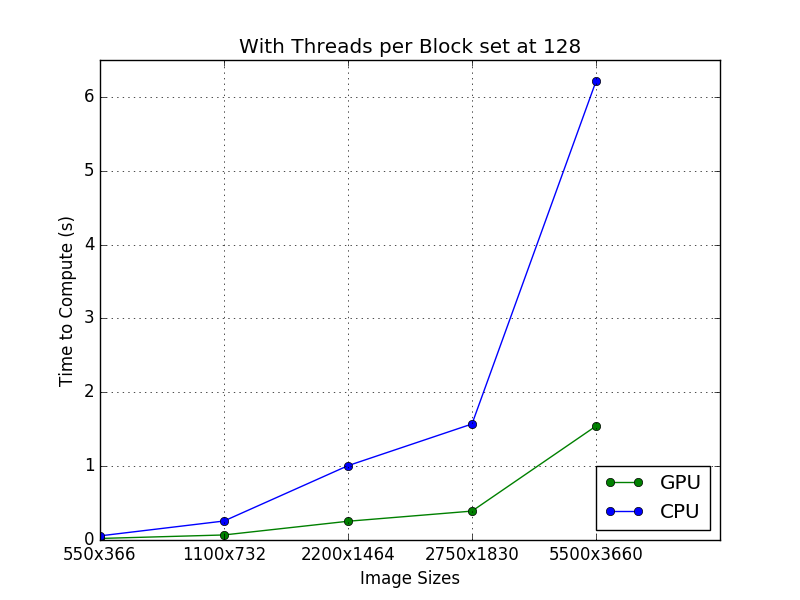
\includegraphics{SizeTime}
\IEEEPARstart{T}{he} rising availability of technology significantly impacts on the way we interact with everything around us, including an increasing consumption of data. Handwriting recognition provides an extremely efficient method for reading data from the physical world. The challenge with implementing a real world handwriting recognition system results from the large variances between how each letter is written. This requires finding a way to correctly classify each of these letters in order to interpret their meaning. In this implementation, multiple 2-class support vector machines are used to accomplish these classifications. To adapt a 2-class SVM to handle a multi-class problem, we have implemented a solution that trains a specific SVM for each class using an all-or-none method. Each SVM will assign the selected class a label of 1 and all other samples a label of -1. Using many bootstrap samples for each of the different classes, we take a mean of the prediction values for each set of bootstrap sample and choose the highest mean value for the selected classification.\\

Reference \cite{BishopBook} clearly showed the fundamental equations and a good understanding of the mechanics behind implementing the SVM.\\

Reference \cite{TullochSVMpy} gave an overview of a SVM implementation which gave great insight into first step to understanding the problem of creating a full SVM implementation.\\

Reference \cite{QuadraticCVXOPT} was a long introduction to understanding quadratic programming problems as well as forming the constraints to fit into cvxopt solver to find the final values.\\


%\hfill mds

%\hfill August 26, 2015

\section{Implementation}
    Our SVM implementation first uses a parser class to transform the input data.  The parser is able to load and write numpy arrays of the testing and label data.  To transform the label sets for training individual class dividers, the parser sets all labels that are of the current class being trained to 1, and to -1 for the rest of the classes.  Additionally, we created a set of kernel functions to be passed into the SVM instance dynamically, depending on the particular kernel needed.  We packaged the training and prediction functionalities into instances of SVM classes, which additionally store trained variables such as the support vectors and the bias.  This allows us to train and store multiple SVMs.\\

    The SVM class is instantiated with the pre-processed samples (feature vectors), their corresponding labels (1 or -1), the appropriate kernel function, and its necessary parameters (such as $\sigma$ for an RBF function).  In the training function, the support vectors are computed by finding the Gram Matrix, which stores all possible combinations of data points being passed into the kernel. We then solve for the dual form using lagrangian optimization (below), using cvxopt for our quadratic programming solver.

    \subsection{Dual Representation (from Eqn. 7.2 \cite{BishopBook})}
    \begin{equation}
    \mathbf{L} = \sum\limits_{N} a_n - \frac{1}{2} \sum\limits_{n} \sum\limits_{m} a_n a_m t_n t_m \mathbf{K}
    \end{equation}

    In order to use the CVXOPT solver we need to convert the Dual Representation into the standard quadratic programming form shown in equation \ref{eq:quad}.

    \subsection{Quadratic Programming Problem \cite{QuadraticCVXOPT}}
    \begin{equation}
    \label{eq:quad}
    \min_{\mathbf{x}} \frac{1}{2}\mathbf{x}^T\mathbf{P}\mathbf{x} - \mathbf{Q}^T\mathbf{x}
    \end{equation}

    \subsection{Parameters for Quadratic Programming}

    By transforming the dual respresentation we derived the parameters shown in equations \ref{eq:P} and \ref{eq:Q}.

    \begin{eqnarray}
    \label{eq:P}
    P = \sum\limits_{n} \sum\limits_{m} t_n t_m \mathbf{K}\\
    \label{eq:Q}
    Q = \left(\begin{IEEEeqnarraybox*}[][c]{,c/c/c,}
    -1&-1&-1\\
    -1&-1&-1\\
    -1&-1&-1%
    \end{IEEEeqnarraybox*}\right)
    \end{eqnarray}
    \begin{itemize}
    \item Where Q's dimensions are determined by number of samples
    \end{itemize}

    \subsection{Constraints}

    Next we changed the constraints into a form that is necessary for the quadratic programming solver as shown in equations \ref{eq:Gxh}, \ref{eq:Axb}.

    \begin{equation}
    \label{eq:Gxh}
    \mathbf{G} \mathbf{x} \preceq \mathbf{h}
    \end{equation}

    \begin{equation}
    \label{eq:Axb}
    \mathbf{A} \mathbf{x} \leq \mathbf{b}
    \end{equation}

    Equation \ref{eq:stdConstraints} is referencing the transformation for the standard constraints.

    \begin{equation}
    \label{eq:stdConstraints}
    a_n \geq 0 \rightarrow -a_n \leq 0
    \end{equation}

    \begin{equation}
    std\mathbf{G} \left(\begin{IEEEeqnarraybox*}[][c]{,c/c/c,}
    -1&0&0\\
    0&-1&0\\
    0&0&-1%
    \end{IEEEeqnarraybox*}\right)
    \end{equation}

    \begin{equation}
    std\mathbf{H} \left(\begin{IEEEeqnarraybox*}[][c]{,c/c/c,}
    0&0&0\\
    0&0&0\\
    0&0&0%
    \end{IEEEeqnarraybox*}\right)
    \end{equation}

    Equation \ref{eq:slackConstraints} is referencing the transformation for the slack constraints.

    \begin{equation}
    \label{eq:slackConstraints}
    a_n \leq \mathbf{C}
    \end{equation}

    \begin{equation}
    slack\mathbf{G} \left(\begin{IEEEeqnarraybox*}[][c]{,c/c/c,}
    1&0&0\\
    0&1&0\\
    0&0&1%
    \end{IEEEeqnarraybox*}\right)
    \end{equation}

    \begin{equation}
    slack\mathbf{H} \left(\begin{IEEEeqnarraybox*}[][c]{,c/c/c,}
    \mathbf{C}&\mathbf{C}&\mathbf{C}\\
    \mathbf{C}&\mathbf{C}&\mathbf{C}\\
    \mathbf{C}&\mathbf{C}&\mathbf{C}%
    \end{IEEEeqnarraybox*}\right)
    \end{equation}

    Equation \ref{eq:equalityConstraints} is referencing the transformation for the equality constraints.

    \begin{equation}
    \label{eq:equalityConstraints}
    \sum\limits_{n = 1}^Na_n t_n = 0
    \end{equation}

    \begin{equation}
    \mathbf{A} = \mathbf{y} \left(\begin{IEEEeqnarraybox*}[][c]{,c/c/c,}
    1&1&1\\
    1&1&1\\
    1&1&1%
    \end{IEEEeqnarraybox*}\right)
    \end{equation}

    \begin{equation}
    \mathbf{B} = \left(\begin{IEEEeqnarraybox*}[][c]{,c/c/c,}
    0&0&0\\
    0&0&0\\
    0&0&0%
    \end{IEEEeqnarraybox*}\right)
    \end{equation}

    \subsection{Bias}
    Solving for \textit{a} gives us the indices for the support vectors. These, along with the passed in data, give us the vectors, labels, and weights of the support vectors. We can use all of this information to find the bias and start computing predictions on the functions. The bias is simply computed from the form in equation \ref{eq:bias}:

    \begin{equation}
    \label{eq:bias}
    b = \frac{1}{N_M} \sum\limits_{n \in M} (t_n - \sum\limits_{m \in S} a_m t_m k(\mathbf{x}_n, \mathbf{x}_m))
    \end{equation}

    \subsection{Prediction}
    We now have everything we need to implement the prediction function from equation \ref{eq:prediction}:

    \begin{equation}
    \label{eq:prediction}
    y(\mathbf{x}) = \sum\limits_{n = 1}^N a_n t_n k(\mathbf{x}, \mathbf{x}_n) + b
    \end{equation}

    We also use equation \ref{eq:prediction} to find the bias since it is the same equation when b is zero.\\

    After calling the training function with the data set, labels, and kernel function, we can now call the predict function by passing in a test point.  It will return some value between 1 and -1 which we can use to classify the point.\\

    Next, we tackled the problem of classifying many classes with an SVM that only supports two class classification. To do this we used two different methods for comparison. In both cases we use a 1 vs the rest model in a bootstrapping method. We train a matrix of SVMs in which the columns denote SVMs trained on different classes and the rows denote SVMs of the same class but different subsets of the training data (bootstrap samples). In the first case, we take the arithmetic mean of each set of SVMs for a particular class. The class with the highest overall mean (above a set certainty threshold) will be used for the final label class, as long as it achives a minimum threshold. The certainty threshold ensures that if all committee results are low, the point should be determined unclassified.\\

    The second bootstrapping testing method classifies points based on the mean of the committee votes, weighted by their standard deviations. To do this, we find the standard deviation of the results, and subtract a standard deviation from the arithmetic mean. This helps to lower confidence intervals in situations where a committee’s individual results for a point vary more, and increase confidence when variance is low for a given point. The class with the highest value is once again chosen, given it is below the certainty threshold. \\

    Finally we have implemented a pickling function to write and load the trained SVMs to a file in order to persist the state of the trained SVMs instead of having to train the SVMs on the same training data over and over again. This can be very beneficial for using larger bootstrapping samples or having more classes where it would take a large amount of time to train.\\




\section{Experiments}

In our first run we used an all-or-nothing pipelining approach for the classification.  With this approach, we trained a SVM for each class divider, using class vs. all points not in that class. The goal of this approach was to get a quick and rough estimation of the accuracy of our trained SVMs.  To test this approach, we stopped running a point through the class dividers when a match was returned.  This approach is not ideal, since it could return many false negatives, especially if letters are similar, such as ‘h’ and ‘k’.  This approach also does not give any indication of a confidence interval on any given test point.\\

In our next training/testing approach, we trained using the bootstrapping approach. After the SVMs were all trained using the bootstrapping method, we used a committee approach to determine the best class for each test point.  The goal of this was to gain a good confidence interval on test points.  In order to do this, the SVMs were grouped by classifier, with a set number of  independently trained SVMs per each of the 8 classifiers.  Each test point is run through each of the set number of runs.  The bootstrapping method provided us with two ways to choose an appropriate classifier.  The first approach was to simply take the arithmetic mean of each of the committee results for the classes.  The class with the highest mean (above a set certainty threshold) is chosen.  The certainty threshold ensures that if all committee results are low, the point should be determined unclassified. In the end we found that for our case the bootstrapping actually made the final percentage worse than when training one time with a larger set of the data.\\

In the initial experiments, the SVMs were initially trained on an easier, adjustable data set composed of two populations of Gaussian distributed data in two dimensions. The separation between the two populations and the standard deviation of the Gaussian noise was adjustable, thus making the separability variable. These datasets allowed us to slowly train our SVM on increasingly complex data sets.\\

The next bootstrapping testing method classified points based on the mean of the committee votes, weighted by their standard deviations.  To do this, we found the standard deviation of the results, and subtracted a standard deviation from the arithmetic mean.   This helps to lower confidence intervals in situations where a committee’s individual results for a point vary more, and increase confidence when variance is low for a given point. The class with the highest value is once again chosen, given it is below the certainty threshold.\\

Once this model of the SVM was implemented, we began to optimize our parameters including the tradeoff parameter C, the minimum value for a Lagrange multiplier to act as a support vector, and the variance of the radial basis function used as our kernel. We found that increasing the tradeoff parameter C too much resulted in a slow drop off of our classification percentage, whereas making it too small, caused a sudden dropoff in classification accuracy. The C tradeoff also had a significant impact on the number of support vectors identified; as C got smaller we saw a greater number of support vectors being used in the calculations increased.\\

\section{Conclusion}
After implementing our SVM and optimizing parameters, we were able to consistently achieve classification rates between 65\% and 74\% on randomly chosen test data. In the process of developing this SVM we found that we often wished we could change global parameters like C and the variance of the radial basis function depending on the class of the data; we found that some letters like $k$ were misclassified much more often than others. After all of the experiments we found that having parameters C = 4, 1 for the sigma of the RBF, 75\% of the total dataset and 3 bootstraps. In the end we would have liked to implement a tree style approach that would better classify closely related letters such as “i” and “j” by having a SVM trained on the two letters specifically instead of just 1 vs the rest.


\ifCLASSOPTIONcaptionsoff
  \newpage
\fi

\begin{thebibliography}{1}

\bibitem{BishopBook}
  Bishop, Christopher M. \emph{Pattern Recognition And Machine Learning.} New York: Springer, 2006. Print.

\bibitem{TullochSVMpy}
  Tulloch, Andrew. \emph{A Basic Soft-Margin Kernel SVM Implementation In Python} Tullo.ch. N.p., 2013. Web. 24 Mar. 2016.

\bibitem{QuadraticCVXOPT}
  \emph{Quadratic Programming With Python And CVXOPT. N.p., 2016. Web. 24 Mar. 2016.}

\end{thebibliography}

\end{document}